% =====================================================================
%  IEEE conference paper (IEEEtran, conference mode, A4)
%  Build:  cd paper && latexmk -pdf main.tex      (system TeX Live)
%     or:  conda run -n tex tectonic main.tex     (no installation needed)
%  All numbers in tables/figures come from src/paper_assets.py.
% =====================================================================
\documentclass[conference,a4paper]{IEEEtran}
\IEEEoverridecommandlockouts
\usepackage{cite}
\usepackage{amsmath,amssymb}
\usepackage{graphicx}
\usepackage{booktabs}
\usepackage{xcolor}
\usepackage{url}
\usepackage{array}
\newcolumntype{L}[1]{>{\raggedright\arraybackslash}p{#1}}
\newcommand{\todo}[1]{\textcolor{red}{[TODO: #1]}}

\begin{document}

\title{Where Does Label Noise Hurt Ensembles? A 0-1 Bias--Variance Decomposition of Bagging, Random Forests and Boosting under Symmetric, One-Sided and Boundary Label Noise}

\author{
\IEEEauthorblockN{Krish Kalola}
\IEEEauthorblockA{\textit{Department of Computer Science} \\
\textit{Pandit Deendayal Energy University}\\
Gandhinagar, Gujarat, India \\
krishkalola@outlook.com}
\and
\IEEEauthorblockN{Harshi Jain}
\IEEEauthorblockA{\textit{Department of Computer Science} \\
\textit{Pandit Deendayal Energy University}\\
Gandhinagar, Gujarat, India \\
harshi.r.jain2005@gmail.com}
\and
\IEEEauthorblockN{Pearl Kalariya}
\IEEEauthorblockA{\textit{Department of Computer Science} \\
\textit{Pandit Deendayal Energy University}\\
Gandhinagar, Gujarat, India \\
pearlkalariyaofficial@gmail.com}
}

\maketitle

% IEEE: abstract 150--250 words, one paragraph, no citations, symbols or equations.
\begin{abstract}
Tree ensembles are the default choice for tabular classification, yet real training labels often contain errors. Earlier studies report how much accuracy ensembles lose under label noise, but not whether the extra error comes from learning a wrong decision rule (bias) or from instability (variance), and they mostly flip labels at random. We measure this directly. On 15 binary datasets selected by a fixed rule from the OpenML-CC18 benchmark, we inject symmetric, one-sided and boundary label noise at rates up to 30 percent and decompose the clean-test error of a decision tree, bagging, random forest, AdaBoost, gradient boosting and XGBoost into bias and variance with the zero-one loss decomposition of Domingos. Symmetric noise adds almost only variance. One-sided noise adds mainly bias to shallow boosted models but mainly variance to deep trees, so the type of damage depends on both the noise and the model capacity. Boundary noise splits roughly evenly and concentrates its damage near the decision boundary. Boosting appears more robust than bagging under default settings, but a capacity-controlled experiment shows that this is a tree-depth effect: at equal depth, bagging and random forests are significantly more robust. Variance-reducing remedies such as small-sample bagging and early stopping recover up to 56 percent of the damage from symmetric noise but no significant share of the damage from one-sided noise. A check on 20 multiclass datasets confirms the patterns for symmetric and boundary noise. Matching the remedy to the noise type therefore matters more than the choice of ensemble.
\end{abstract}

\begin{IEEEkeywords}
label noise, ensemble learning, bias--variance decomposition, bagging, boosting, random forest
\end{IEEEkeywords}

% ---------------------------------------------------------------------
\section{Introduction}
Tree-based ensembles such as bagging \cite{breiman1996}, random forests \cite{breiman2001} and boosting \cite{freund1997,friedman2001,chen2016} remain the strongest general-purpose models for tabular data. In practice their training labels are rarely perfect: annotators make mistakes, ambiguous cases are labelled inconsistently and automated labelling introduces systematic errors \cite{frenay2014}. It is therefore important to know how label noise affects each kind of ensemble.

Much is already known about \emph{how much} noise hurts. Dietterich \cite{dietterich2000} showed that bagging is more robust than boosting when labels are flipped at random, and recent work shows that the robustness ranking of modern gradient-boosting libraries depends on the type of noise \cite{morampudi2026}. These studies, however, report only accuracy-type degradation. They do not say \emph{why} an ensemble degrades: does noise make the model learn a systematically wrong rule (bias), or does it make the model unstable (variance)? The answer is practically important, because the two problems need opposite remedies. Variance can be reduced by averaging or early stopping; bias caused by wrong labels can only be removed by correcting the data.

This paper measures the answer. We combine controlled label-noise injection with the zero-one loss bias--variance decomposition of Domingos \cite{domingos2000} and ask four questions:
\begin{itemize}
\item \textbf{RQ1:} How does each ensemble's error grow with the noise rate?
\item \textbf{RQ2:} Is the extra error mainly bias or variance, and does this depend on the noise type and the ensemble family?
\item \textbf{RQ3:} Does the noise-induced variance come from \emph{which} labels are flipped or from \emph{which} rows are sampled?
\item \textbf{RQ4:} Do standard regularisation remedies recover the damage under every noise type?
\item \textbf{RQ5:} Do the binary findings still hold for multiclass data?
\end{itemize}

Our contributions are: (i) the first measured bias--variance attribution of noise-induced error across parallel and sequential tree ensembles under symmetric, one-sided and boundary noise; (ii) evidence for one-sided class-conditional noise on binary tasks, a setting left open by recent work \cite{morampudi2026}; (iii) a capacity-controlled experiment showing that the apparent robustness of boosting under default settings is a tree-depth effect; (iv) practical guidance that matches remedies to noise types; and (v) a check on 20 multiclass datasets showing which findings generalise beyond binary tasks. All code and results are released for reproducibility \todo{GitHub link}.

% ---------------------------------------------------------------------
\section{Background}

\subsection{Tree Ensembles}
Bagging trains each tree on a bootstrap sample and combines them by majority vote \cite{breiman1996}; random forests additionally sample features at each split \cite{breiman2001}. Both are \emph{parallel} ensembles whose main effect is variance reduction. AdaBoost \cite{freund1997} and gradient boosting \cite{friedman2001,chen2016} are \emph{sequential}: each new tree concentrates on the examples that earlier trees got wrong, which mainly reduces bias but can also make the ensemble chase mislabelled examples \cite{long2010}.

\subsection{Label-Noise Types}
Following the taxonomy of Fr\'enay and Verleysen \cite{frenay2014}, we study three noise types. \emph{Symmetric} noise flips labels completely at random (NCAR). \emph{One-sided} noise flips only class~1 to class~0, a class-conditional model (NAR) \cite{natarajan2013} that describes, for example, missed diagnoses. \emph{Boundary} noise flips mainly examples near the decision boundary, an instance-dependent model (NNAR) that reflects human errors on ambiguous cases \cite{saez2022}.

\subsection{Zero-One Loss Bias--Variance Decomposition}
Let a learner be trained $R$ times on different training samples and let $\hat{y}_r(x)$ be the prediction of the $r$-th model for a test point $x$ with true label $y$. Following \cite{domingos2000}, the \emph{main prediction} $y_m(x)$ is the majority vote of the $R$ models, the bias is $B(x)=\mathbb{1}[y_m(x)\neq y]$ and the variance is $V(x)=\Pr_r[\hat{y}_r(x)\neq y_m(x)]$. For binary labels and noise-free test labels the expected loss is
\begin{equation}
\mathbb{E}[L(x)] = B(x) + \bigl(1-2B(x)\bigr)\,V(x). \label{eq:domingos}
\end{equation}
Variance therefore \emph{adds} to the error where the main prediction is correct (unbiased variance) and \emph{subtracts} from it where the main prediction is wrong (biased variance). Averaged over the test set,
\begin{equation}
\text{error} = \text{bias} + \underbrace{V_u - V_b}_{\text{net variance}},
\end{equation}
where $V_u$ and $V_b$ are the average unbiased and biased variance. We report the bias and the net variance, which add up exactly to the error.

% ---------------------------------------------------------------------
\section{Related Work}
Dietterich \cite{dietterich2000} compared bagging, boosting and randomisation of C4.5 trees and found bagging much better under random classification noise. Khoshgoftaar \emph{et al.} \cite{khoshgoftaar2011} reached a similar conclusion for noisy, imbalanced binary data. Long and Servedio \cite{long2010} proved that random classification noise can defeat any convex-potential booster, even with early stopping. Sabzevari \emph{et al.} \cite{sabzevari2015} showed that bagging with small bootstrap samples is more robust to label noise, and S\'aez and Romero-B\'ejar \cite{saez2022} studied bagging under borderline noise. Eisenb\"urger \emph{et al.} \cite{eisenburger2024} studied noise detection for gradient-boosted trees, and Morampudi \emph{et al.} \cite{morampudi2026} showed that the robustness ranking of XGBoost, LightGBM and CatBoost depends on the noise model; they measured only accuracy-type metrics and explicitly left one-sided binary noise and remedies under non-symmetric noise open. On the theory side, Wood \emph{et al.} \cite{wood2023} unified bias, variance and diversity in ensembles, and He \emph{et al.} \cite{he2026} used this framework to design noise-robust ensemble algorithms. Mohammad \cite{mohammad2025} discussed ensembles on tabular data from a bias--variance perspective but without injected noise or a formal decomposition. To our knowledge no study \emph{measures} how noise-induced error splits into bias and variance across noise types and ensemble families.
\todo{After reading the full text of He et al. (2026), confirm this last sentence.}

% ---------------------------------------------------------------------
\section{Experimental Setup}

\subsection{Datasets}
To avoid hand-picking, we used \emph{all} binary datasets of the OpenML-CC18 benchmark \cite{vanschoren2014,bischl2021} with at most 50{,}000 rows, at most 100 features, no missing values and a minority class of at least 15\%. Of the 35 binary CC18 datasets, 15 satisfy the rule (Table~\ref{tab:datasets}). Labels were coded so that the minority class is class~1. Each dataset was split once into a stratified 70\% training pool and a 30\% test set; categorical features were one-hot encoded using the training part only. Label noise was injected into training labels only, so all errors are measured against clean test labels.

\begin{table}[!t]
\caption{Datasets (OpenML-CC18), Ordered by Size. Pos.\ Is the Share of Class~1.}
\label{tab:datasets}
\centering
\footnotesize
\begin{tabular}{@{}lrrrr@{}}
\toprule
Dataset & ID & Rows & Feat. & Pos. \\
\midrule
kc2 & 1063 & 522 & 21 & 0.20 \\
wdbc & 1510 & 569 & 30 & 0.37 \\
ilpd & 1480 & 583 & 11 & 0.29 \\
blood-transfusion & 1464 & 748 & 4 & 0.24 \\
diabetes & 37 & 768 & 8 & 0.35 \\
tic-tac-toe & 50 & 958 & 27 & 0.35 \\
credit-g & 31 & 1,000 & 61 & 0.30 \\
qsar-biodeg & 1494 & 1,055 & 41 & 0.34 \\
banknote-authentication & 1462 & 1,372 & 4 & 0.45 \\
kc1 & 1067 & 2,109 & 21 & 0.15 \\
kr-vs-kp & 3 & 3,196 & 73 & 0.48 \\
spambase & 44 & 4,601 & 57 & 0.39 \\
phoneme & 1489 & 5,404 & 5 & 0.29 \\
PhishingWebsites & 4534 & 11,055 & 68 & 0.44 \\
electricity & 151 & 45,312 & 14 & 0.42 \\
\bottomrule
\end{tabular}
\end{table}

\subsection{Models}
We compared six classifiers implemented in scikit-learn \cite{pedregosa2011} and XGBoost \cite{chen2016}: an unpruned decision tree; bagging and a random forest, each with 100 unpruned trees; AdaBoost with 100 decision stumps; gradient boosting (GB) with 100 trees of depth~3 and learning rate 0.1; and XGBoost (XGB) with 100 trees of depth~4 and learning rate 0.1. Hyperparameters were fixed and identical in every noise condition, so that changes in error are caused by the noise alone.

\subsection{Noise Injection}
For a rate $\rho$, symmetric noise flips exactly $\rho n$ labels chosen uniformly at random. One-sided noise flips exactly $\rho n_1$ labels of class~1 to class~0, where $n_1$ is the number of positives. Boundary noise flips exactly $\rho n$ labels, choosing each example with probability proportional to $1-2|p(x)-0.5|$, where $p(x)$ is the class-1 probability of a logistic regression trained on the clean labels. We used $\rho\in\{5,10,20,30\}\%$.

\subsection{Protocol}
For every dataset, model, noise type and rate, the model was trained $R=51$ times, each time on a fresh bootstrap sample of the training pool with freshly injected noise, and evaluated on the clean test set. An odd $R$ avoids ties in the majority vote. The bootstrap sample and noise mask of round $r$ depend only on the round, not on the model, so all models face identical training data (common random numbers), and every comparison between models is paired. The main grid has 15 datasets, 6 models and 13 noise conditions (clean, and three noise types at four rates), giving 1{,}170 conditions and about 60{,}000 model fits. The \emph{damage} caused by noise is the change in error, bias and net variance relative to the same model on clean labels; by construction $\Delta\text{error}=\Delta\text{bias}+\Delta\text{net variance}$.

\subsection{Additional Experiments}
Three further experiments reuse the same datasets, seeds and protocol at rates of 10, 20 and 30\%.

\emph{Capacity control.} Under default settings the parallel ensembles grow full-depth trees, whereas AdaBoost uses stumps and GB and XGB use trees of depth 3 and 4. To separate the ensemble method from tree size, we added depth-matched variants: bagging, random forest, AdaBoost and XGB with depth-3 trees, and GB and XGB with depth-8 trees.

\emph{Sources of variance (RQ3).} At 20\% noise, each model was additionally trained under three designs that re-draw only part of the randomness: only the model's own random seed (training rows and noise mask fixed), only the noise mask (training rows fixed) and only the bootstrap sample (noise mask fixed). Subtracting the variance of the first design from the other two gives the variance added by the noise realisation and by sampling.

\emph{Remedies (RQ4).} Each of four standard remedies was compared with its base model: GB and XGB with learning rate 0.05, 80\% row subsampling and early stopping on a 10\% split of the (noisy) training data; AdaBoost with learning rate 0.5; and bagging with bootstrap samples of 20\% of the training set \cite{sabzevari2015}. The \emph{damage recovered} is $1-\Delta\text{error}_{\text{remedy}}/\Delta\text{error}_{\text{base}}$.

Finally, to see \emph{where} the damage lands, each test set was split at the median of the margin $|p(x)-0.5|$ of the clean logistic-regression reference into a near-boundary and a far-from-boundary half, and the saved predictions of the main grid were decomposed separately in each half.

\subsection{Multiclass Extension (RQ5)}
Applying the same selection rule to the multiclass datasets of OpenML-CC18 (with a smallest class of at least 5\%) yields 20 datasets with 3 to 11 classes, prepared exactly as the binary ones. Symmetric noise moves a flipped label to a uniformly chosen other class. As the multiclass counterpart of one-sided noise we use \emph{pair-flip} noise, which moves class $k$ to class $k+1$ (classes ordered by frequency). Boundary noise selects examples with probability proportional to one minus the top-class probability of a multinomial logistic-regression reference and moves each to the reference's most likely other class. With $K>2$ classes, a model that disagrees with a wrong main prediction lowers the error only if it predicts the true class, so the biased variance in the decomposition is replaced by the probability of predicting the true class at biased points; the identity $\text{error}=\text{bias}+\text{net variance}$ still holds exactly and reduces to (1) for $K=2$. Rates of 10, 20 and 30\% and the same six models and protocol were used.

\subsection{Statistical Analysis}
Following Dem\v{s}ar \cite{demsar2006}, models were compared over the 15 datasets with the Friedman test on their ranks, followed by the Nemenyi critical difference (CD) at $\alpha=0.05$; pairs of models were compared with the Wilcoxon signed-rank test.

% ---------------------------------------------------------------------
\section{Results}

\subsection{RQ1: How Much Does Noise Hurt?}
Fig.~\ref{fig:rq1} shows the average increase in test error. The single tree is hurt most under every noise type. With default settings the sequential ensembles lose less accuracy than the parallel ones under symmetric and boundary noise: at 30\% symmetric noise the error of bagging rises by 11.7 percentage points (pp) and that of random forest by 10.9~pp, against 4.3~pp for AdaBoost and 7.6~pp for GB. At equal rate, one-sided noise is the mildest type for every model except AdaBoost, which is hurt slightly more by one-sided than by symmetric noise.

Table~\ref{tab:ranks} ranks the models by damage on each dataset. Under symmetric and boundary noise the differences are highly significant (Friedman $p<10^{-5}$). AdaBoost has the best average rank, and with a CD of 1.95 its advantage over the single tree and bagging is significant. Under one-sided noise, in contrast, no model is consistently more robust ($p=0.48$): the choice of ensemble does not protect against one-sided noise. Section~\ref{sec:capacity} shows that the advantage of boosting under the other two noise types is explained by tree depth.

\begin{figure*}[!t]
\centering
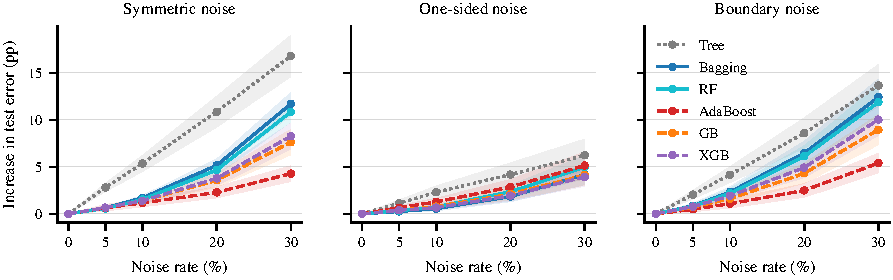
\includegraphics[width=\textwidth]{figures/fig_rq1_error_vs_noise.pdf}
\caption{Increase in clean-test error caused by label noise, averaged over 15 datasets (shaded: $\pm$1 standard error).}
\label{fig:rq1}
\end{figure*}

\begin{table}[!t]
\caption{Average Rank of Damage at 20\% Noise Over 15 Datasets (1 = Least Damaged)}
\label{tab:ranks}
\centering
\footnotesize
\begin{tabular}{@{}lrrr@{}}
\toprule
Model & Sym. & One-s. & Bound. \\
\midrule
Tree & 5.60 & 3.53 & 5.27 \\
Bagging & 3.87 & 2.73 & 4.13 \\
RF & 3.40 & 4.07 & 3.73 \\
AdaBoost & 1.73 & 3.67 & 1.33 \\
GB & 3.13 & 3.73 & 2.80 \\
XGB & 3.27 & 3.27 & 3.73 \\
\midrule
Friedman $p$ & 2.7e-06 & 0.482 & 4.2e-07 \\
\bottomrule
\end{tabular}
\end{table}

\subsection{RQ2: Bias or Variance?}
Fig.~\ref{fig:rq2} and Table~\ref{tab:rq2} split the damage at 20\% noise. Under \emph{symmetric} noise the damage is almost pure variance (96--105\% of the damage for every model except AdaBoost, 71\%): random flips do not move the learned rule on average, they make it unstable. Under \emph{one-sided} noise the picture depends on the model. For the shallow boosted models the damage is mainly bias (variance share 7\% for AdaBoost and 17\% for GB), because removing positives shifts the learned decision rule towards class~0. For the deep single tree and bagging it remains mainly variance (94\% and 89\%). Under \emph{boundary} noise the damage is split roughly evenly (37--54\% variance), and the share of bias grows with the noise rate. A variance share above 100\% means that bias decreased slightly while variance increased.

\begin{figure*}[!t]
\centering
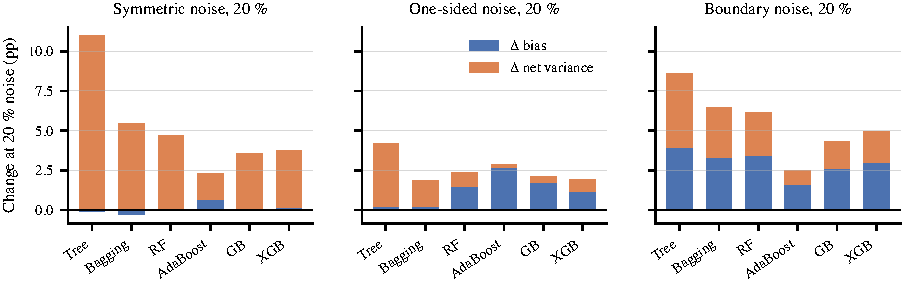
\includegraphics[width=\textwidth]{figures/fig_rq2_bias_variance.pdf}
\caption{Damage at 20\% noise split into change in bias and change in net variance (averages over 15 datasets).}
\label{fig:rq2}
\end{figure*}

\begin{table}[!t]
\caption{Damage at 20\% Noise (pp) and the Share Due to Variance}
\label{tab:rq2}
\centering
\footnotesize
\begin{tabular}{@{}lrrrr@{}}
\toprule
Model & $\Delta$err & $\Delta$bias & $\Delta$var & Var.\ share \\
\midrule
\multicolumn{5}{@{}l}{\emph{Symmetric noise}} \\
Tree & 10.9 & $-$0.1 & 11.0 & 101\% \\
Bagging & 5.2 & $-$0.3 & 5.4 & 105\% \\
RF & 4.7 & 0.1 & 4.6 & 99\% \\
AdaBoost & 2.3 & 0.7 & 1.6 & 71\% \\
GB & 3.6 & 0.1 & 3.5 & 98\% \\
XGB & 3.8 & 0.2 & 3.6 & 96\% \\
\multicolumn{5}{@{}l}{\emph{One-sided noise}} \\
Tree & 4.2 & 0.2 & 3.9 & 94\% \\
Bagging & 1.8 & 0.2 & 1.6 & 89\% \\
RF & 2.4 & 1.5 & 0.9 & 36\% \\
AdaBoost & 2.9 & 2.6 & 0.2 & 7\% \\
GB & 2.1 & 1.8 & 0.3 & 17\% \\
XGB & 1.9 & 1.2 & 0.8 & 40\% \\
\multicolumn{5}{@{}l}{\emph{Boundary noise}} \\
Tree & 8.6 & 3.9 & 4.7 & 54\% \\
Bagging & 6.5 & 3.3 & 3.2 & 49\% \\
RF & 6.1 & 3.4 & 2.7 & 44\% \\
AdaBoost & 2.5 & 1.6 & 0.9 & 37\% \\
GB & 4.3 & 2.6 & 1.7 & 40\% \\
XGB & 4.9 & 3.0 & 1.9 & 39\% \\
\bottomrule
\end{tabular}
\end{table}

\subsection{Capacity Control: Ensemble Method or Tree Size?}\label{sec:capacity}
Fig.~\ref{fig:capacity} shows that deeper trees are damaged more in every family under symmetric and boundary noise (all $p<0.03$). At equal depth the ordering of RQ1 reverses: depth-3 bagging and random forests are damaged 2.5--5.0~pp \emph{less} than depth-3 boosting under symmetric and boundary noise (Table~\ref{tab:cap}, all $p<0.001$). This agrees with Dietterich \cite{dietterich2000}, whose boosted trees were also deep, and shows that the apparent robustness of boosting in RQ1 is a tree-depth effect. Under one-sided noise tree depth makes no significant difference, consistent with its bias-type damage. Depth also changes the \emph{type} of one-sided damage: its variance share rises from 17\% for GB with depth-3 trees to 89\% with depth-8 trees. Shallow bagging has, however, a higher clean error (18.0\% against 13.6\% for full-depth bagging), so being least damaged is not the same as being most accurate under noise.

\begin{figure*}[!t]
\centering
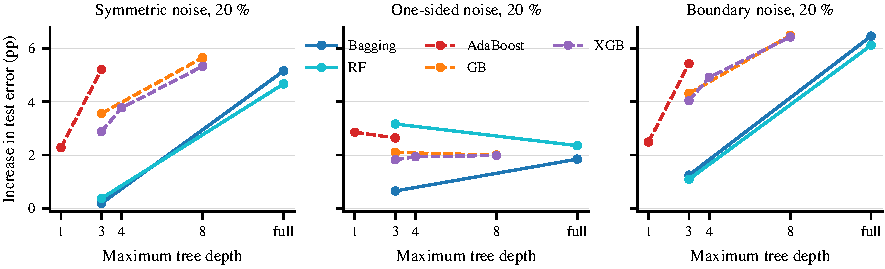
\includegraphics[width=\textwidth]{figures/fig_capacity_depth.pdf}
\caption{Damage at 20\% noise as a function of maximum tree depth for each ensemble family.}
\label{fig:capacity}
\end{figure*}

\begin{table}[!t]
\caption{Damage Difference at Equal Depth (pp, Parallel Minus Sequential, 20\% Noise). $^{*}$: $p<0.05$, Wilcoxon}
\label{tab:cap}
\centering
\footnotesize
\begin{tabular}{@{}llrrr@{}}
\toprule
Parallel & Sequential & Sym. & One-s. & Bound. \\
\midrule
Bagging\_d3 & AdaBoost\_d3 & $-$5.0$^{*}$ & $-$2.0$^{*}$ & $-$4.2$^{*}$ \\
Bagging\_d3 & GB & $-$3.4$^{*}$ & $-$1.4$^{*}$ & $-$3.1$^{*}$ \\
Bagging\_d3 & XGB\_d3 & $-$2.7$^{*}$ & $-$1.2$^{*}$ & $-$2.8$^{*}$ \\
RF\_d3 & AdaBoost\_d3 & $-$4.8$^{*}$ & 0.5 & $-$4.3$^{*}$ \\
RF\_d3 & GB & $-$3.2$^{*}$ & 1.1 & $-$3.2$^{*}$ \\
RF\_d3 & XGB\_d3 & $-$2.5$^{*}$ & 1.3 & $-$2.9$^{*}$ \\
\bottomrule
\end{tabular}
\end{table}

\subsection{RQ3: Where Does the Variance Come From?}
Table~\ref{tab:rq3} shows that the noise realisation and sampling add similar amounts of variance in most cases. Under boundary noise, however, the choice of flipped labels contributes more than resampling for bagging and random forests (9.6 vs.\ 7.5~pp and 8.1 vs.\ 5.8~pp). Averaging over bootstrap samples cannot remove this part, because every tree in the ensemble sees the same wrong labels. The boosting models have almost no variance of their own, whereas bagging and random forests have 2--4~pp from their internal randomness.

\begin{table}[!t]
\caption{Variance Added by the Noise Realisation and by Sampling (pp, 20\% Noise)}
\label{tab:rq3}
\centering
\footnotesize
\setlength{\tabcolsep}{4pt}
\begin{tabular}{@{}lrrrrrr@{}}
\toprule
 & \multicolumn{2}{c}{Symmetric} & \multicolumn{2}{c}{One-sided} & \multicolumn{2}{c}{Boundary} \\
\cmidrule(lr){2-3}\cmidrule(lr){4-5}\cmidrule(lr){6-7}
Model & Noise & Samp. & Noise & Samp. & Noise & Samp. \\
\midrule
Tree & 20.4 & 19.4 & 11.2 & 11.5 & 17.1 & 15.2 \\
Bagging & 9.0 & 9.0 & 4.1 & 5.2 & 9.6 & 7.5 \\
RF & 7.8 & 7.3 & 3.2 & 3.7 & 8.1 & 5.8 \\
AdaBoost & 8.3 & 9.1 & 4.3 & 5.3 & 7.8 & 7.9 \\
GB & 9.5 & 10.4 & 4.6 & 5.7 & 9.3 & 8.6 \\
XGB & 10.2 & 11.0 & 5.0 & 6.1 & 10.2 & 9.4 \\
\bottomrule
\end{tabular}
\end{table}

\subsection{Where Does the Damage Land?}
Table~\ref{tab:margin} compares the damage in the near-boundary and far-from-boundary halves of the test sets. Boundary noise concentrates its damage near the boundary, 10 to 18 times more for the ensembles; one-sided noise does so moderately for boosting (about 3.7 times); and symmetric noise spreads it roughly evenly. For the single tree, symmetric noise even causes more damage far from the boundary (ratio 0.7), because a full-depth tree memorises flipped labels in otherwise confident regions.

\begin{table}[!t]
\caption{Ratio of Damage Near vs.\ Far From the Decision Boundary (20\% Noise)}
\label{tab:margin}
\centering
\footnotesize
\begin{tabular}{@{}lrrr@{}}
\toprule
Model & Sym. & One-s. & Bound. \\
\midrule
Tree & 0.7 & 1.1 & 3.7 \\
Bagging & 1.0 & 1.8 & 10.2 \\
RF & 1.2 & 2.0 & 11.0 \\
AdaBoost & 1.5 & 3.8 & 17.9 \\
GB & 1.3 & 3.6 & 10.0 \\
XGB & 1.5 & 3.7 & 10.7 \\
\bottomrule
\end{tabular}
\end{table}

\subsection{RQ4: Do Common Remedies Help?}
Table~\ref{tab:rq4} reports the share of the noise damage recovered by each remedy. Variance-reducing remedies work under symmetric and boundary noise: training bagging on 20\% bootstrap samples recovers 56\% and 33\% of the damage (better on 14 of 15 datasets), and early stopping with a lower learning rate recovers about 19\% for GB and XGB while also slightly lowering their clean error. Under one-sided noise none of the remedies helps significantly, and early stopping even increases the damage by about 11\%. This is consistent with RQ2, since one-sided damage is mainly bias, which averaging and early stopping cannot correct, and with the theory of Long and Servedio \cite{long2010}. The lower learning rate for AdaBoost reduces the damage but costs about 1~pp of clean accuracy, so its error under noise does not improve significantly.

\begin{table}[!t]
\caption{Share of Noise Damage Recovered by Each Remedy (20\% Noise). $^{*}$: Noisy Error Significantly Lower, $p<0.05$}
\label{tab:rq4}
\centering
\footnotesize
\begin{tabular}{@{}lrrr@{}}
\toprule
Fix & Sym. & One-s. & Bound. \\
\midrule
GB, early stop & 19\%$^{*}$ & $-$11\% & 7\%$^{*}$ \\
XGB, early stop & 19\%$^{*}$ & $-$11\% & 8\%$^{*}$ \\
AdaBoost, $\eta{=}0.5$ & 36\% & 14\% & 28\% \\
Bagging, 20\% samples & 56\%$^{*}$ & 6\% & 33\%$^{*}$ \\
\bottomrule
\end{tabular}
\end{table}

\subsection{RQ5: Do the Findings Hold for Multiclass Data?}
Table~\ref{tab:multiclass} repeats the split of RQ2 on the 20 multiclass datasets. The two central findings carry over. Symmetric noise again adds almost only variance (variance share 103--131\% for all models but AdaBoost), and boundary noise again splits roughly evenly (51--70\% variance) with the bias share growing with the noise rate. For class-conditional (pair-flip) noise, stump-based AdaBoost is again almost pure bias (5\%), whereas GB and XGB are now mostly variance (75--83\%). This agrees with the capacity effect of Section~\ref{sec:capacity}: class-conditional noise produces bias in low-capacity models and variance in higher-capacity ones. Unlike binary one-sided noise, the models differ significantly under pair-flip noise (Friedman $p<10^{-6}$), and random forests and bagging have the best average damage ranks (2.2 and 2.6). Symmetric noise hurts the ensembles less than in the binary case (2--3~pp at 20\%), because flips spread over many wrong classes rarely outvote the true class. AdaBoost with stumps fits multiclass data poorly (clean error 33\% against about 20\% for the other ensembles), and its error even falls slightly under symmetric noise, so its multiclass results should be read with caution.

\begin{table}[!t]
\caption{Multiclass Datasets: Damage at 20\% Noise (pp) and Share Due to Variance}
\label{tab:multiclass}
\centering
\footnotesize
\setlength{\tabcolsep}{4pt}
\begin{tabular}{@{}lrrrrrr@{}}
\toprule
 & \multicolumn{2}{c}{Symmetric} & \multicolumn{2}{c}{Pair-flip} & \multicolumn{2}{c}{Boundary} \\
\cmidrule(lr){2-3}\cmidrule(lr){4-5}\cmidrule(lr){6-7}
Model & $\Delta$err & Var. & $\Delta$err & Var. & $\Delta$err & Var. \\
\midrule
Tree & 13.0 & 103\% & 10.9 & 103\% & 8.4 & 70\% \\
Bagging & 1.8 & 131\% & 3.5 & 99\% & 4.1 & 59\% \\
RF & 1.9 & 104\% & 3.3 & 94\% & 4.2 & 55\% \\
AdaBoost & $-$2.2 & -- & 8.0 & 5\% & 1.8 & 56\% \\
GB & 3.3 & 106\% & 5.2 & 83\% & 4.1 & 52\% \\
XGB & 2.2 & 114\% & 4.3 & 75\% & 3.7 & 51\% \\
\bottomrule
\end{tabular}
\end{table}

% ---------------------------------------------------------------------
\section{Discussion}
The results lead to a simple practical rule, summarised in Table~\ref{tab:guide}: identify the likely type of label error from how the labels were produced, and choose the remedy accordingly. Random errors, such as data-entry slips, cause variance, which variance-reducing ensembles and regularisation can control. One-sided errors, such as under-reported positives, shift the decision rule; here the choice of ensemble does not matter significantly and regularisation does not help, so effort should go into correcting labels or re-weighting the affected class. Errors on ambiguous cases cause both kinds of damage and concentrate it on borderline test points, so both kinds of remedy are needed.

The capacity experiment carries a methodological lesson: comparing ensemble families under default settings mixes the combination method with tree size. Under default settings boosting looked the most robust, but at equal depth the classic result of Dietterich \cite{dietterich2000} holds.

\begin{table}[!t]
\caption{Practical Guide Derived From the Results}
\label{tab:guide}
\centering
\footnotesize
\setlength{\tabcolsep}{3pt}
\begin{tabular}{@{}L{1.45cm}L{1.6cm}L{1.75cm}L{2.05cm}@{}}
\toprule
Likely noise & Main damage & Model choice & Remedy \\
\midrule
Random (symmetric) & Variance & Parallel ensemble with limited depth & Small-sample bagging, early stopping \\
One-sided & Bias (shallow), variance (deep) & No significant difference & Correct or re-weight labels; regularisation does not help \\
Ambiguous cases (boundary) & Bias and variance, near boundary & Parallel ensemble with limited depth & Variance reduction plus label review of borderline cases \\
\bottomrule
\end{tabular}
\end{table}

\section{Limitations}
The main study uses binary tasks; the multiclass check covers fewer remedies and a single class-conditional pattern (pair-flip). All experiments use tree-based ensembles and synthetic label noise injected at controlled rates, whereas real noise may combine several types. Hyperparameters were fixed and not re-tuned for each noise level. Boundary noise was defined with a logistic-regression reference, which favours linear decision boundaries. The variance estimates use bootstrap samples from one training pool, which slightly understates the variance across independently drawn training sets.

\section{Conclusion}
Label noise does not damage all tree ensembles in the same way. Random noise mainly adds variance; one-sided noise adds bias to low-capacity models and variance to high-capacity ones; boundary noise adds both and concentrates near the decision boundary. At equal tree depth bagging and random forests are more robust than boosting, variance-reducing remedies help only when the damage is variance, and the main patterns also hold on multiclass data. Choosing the remedy according to the likely type of label error is therefore the key practical decision.

\section*{Acknowledgment}
\todo{Thank your guide/department, if appropriate.}
\todo{AI disclosure required by IEEE policy: name the AI tool used and state which parts it assisted with (e.g., code for the experiments, figure scripts, drafting or editing of specific sections), and confirm that the authors reviewed and take responsibility for all content.}

\bibliographystyle{IEEEtran}
\bibliography{references}

\end{document}
